\chapter[Governo Digital]{Governo Digital}
Ao iniciarmos esse estudo faz-se necessário a definição do que é o governo digital. Ter conhecimento sobre tal conceito é de extrema relevância, pois nos permite entender o contexto que origina os serviços digitizados e suas formas de avaliação, que é o foco deste trabalho. Além disso é perceptível a importância do assunto e o impacto que pode causar em uma sociedade e em seu governo.

Concordando com \cite{itac2016} para que um governo se mantenha competitivo no cenário mundial e que tenha engajamento dos cidadãos é de crítica importância sua característica digital. Na economia moderna há vantagens na construção de um governo realmente digital, como oportunidades de transformação, modernização e digitização que ajudam no crescimento e na escalabilidade de uma organização.

\subsection{Definição}
Governo digital ou E-GOV foi definido por \cite[p.~2902]{act2002} como: "o uso pelo governo de aplicações baseadas na internet e outras tecnologias de informação, combinadas com processos que implementam essas tecnologias para melhorar o acesso à entregas de serviço feitas ao público, outras agências e outras entidades governamentais; ou trazer melhorias operações governamentais que podem incluir efetividade, eficiência, qualidade de serviço ou transformação."

Outra definição de governo digital, agora de acordo com \cite{itac2016} se baseia em 4 características principais:
\begin{itemize}
	\item A facilidade de se trabalhar com o governo
	\item A facilidade de se trabalhar no governo
	\item As tecnologias são sempre atualizadas 
	\item A informação governamental é digitizada e facilmente encontrável.
\end{itemize}

Portanto são áreas que devem nortear o investimento governamental para se conquistar um governo realmente digital.
 
O Comitê de Governança Pública em sua Recomendação para Estratégias de Governo Digital \cite{oecd2014} destaca as vantagens da adoção das novas tecnologias no governo. Esses valores extrapolam os limites da organização, alcançando o cidadão, as empresas e até organizações não-governamentais. 

O ambiente digital oferece oportunidades para que todos participem de decisões de priorização política, no desenho de serviços públicos e permite que o governo possa antecipar as necessidades dos interessados em seus negócios. A digitização do governo, entretanto, não é instalada por inteiro na estrutura governamental, de acordo com \cite{mckinsey2016} os esforços se iniciam na reconstrução das capacidades básicas com novas tecnologias. 

Com a experiência adquirida dentro da instituição é possível então entregar a experiência de ser digital para os cidadãos, empresas ou qualquer usuário dos serviços disponíveis.

\section{Governo para o cidadão}

\cite[p.~380]{chen2009} ressalta outra perspectiva das iniciativas de governo digial, que podem ser definidas pelo seu público-alvo como visto na Imagem \ref{img:egovdeliverymodel}. Onde:
\begin{itemize}
	\item G2C: Governo para Cidadão;
	\item G2B: Governo para Negócios;
	\item G2G: Governo para Governo;
	\item G2E: Governo para Funcionários;
\end{itemize}

\begin{figure}[hbp]
	\centering
	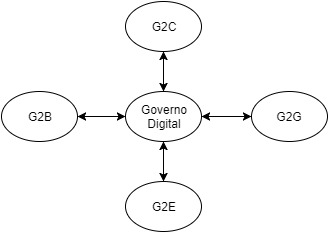
\includegraphics[width=.8\linewidth]{figuras/egovdeliverymodel.jpg}
	\caption{Modelo de entrega de governo digital. Adaptado de \cite{chen2009}}
	\label{img:egovdeliverymodel}
\end{figure}

Para o autor as abordagens acima levantam a necessidade de que 04 (quatro) atividades sejam executadas no governo. 
\begin{itemize}
	\item Disponibilização de informações na internet, como serviços regulatórios, formulários de serviços diversos, agendas de audiências públicas, explicações de processos dos serviços e notificações;
	\item Comunicação bi-lateral com o cidadão, outras agências governamentais ou de negócios, assim o diálogo se torna mais direto e portanto, mais eficiente;
	\item Realizar transações financeiras como retorno de impostos e pagamento de serviços;
	\item Governança, com pesquisas online, votações e campanhas por meios digitais;
\end{itemize}

O governo para o cidadão, dentro do modelo acima, utiliza de uma premissa chamada Gerência da Relação com o Consumidor (CRM) que, de acordo com \cite{larsen2005}, é uma estratégia de negócios com o foco no lucro, que direciona as empresas a melhor servirem o consumidor\footnote{Na visão do CRM o consumidor é um indivíduo com um conjunto único de interesses e necessidades, tem o direito de receber um serviço customizado, rápido e conveniente. Portanto, serviços como \textit{internet banking} e \textit{e-commerce} se adequam à esse perfil, onde o consumidor tem esse tratamento a seu dispor com as tecnologias \textit{self-service}.} de forma a melhorar o entendimento de suas necessidades e desejos.

As mudanças ocasionadas pela transformação dos consumidores, de compradores passivos para co-desenvolvedores com experiências personalizadas, forçaram a mudança de como as empresas fornecem informações, serviços e como interagem com seus consumidores. 
